%% LyX 2.2.2 created this file.  For more info, see http://www.lyx.org/.
%% Do not edit unless you really know what you are doing.
\documentclass[UTF8]{ctexart}
\usepackage{fontspec}
\usepackage{geometry}
\geometry{verbose,tmargin=2.54cm,bmargin=2.54cm,lmargin=3.18cm,rmargin=3.18cm}
\pagestyle{plain}
\usepackage{graphicx}
\usepackage[unicode=true,pdfusetitle,
 bookmarks=true,bookmarksnumbered=true,bookmarksopen=true,bookmarksopenlevel=1,
 breaklinks=false,pdfborder={0 0 1},backref=false,colorlinks=false]
 {hyperref}

\makeatletter

%%%%%%%%%%%%%%%%%%%%%%%%%%%%%% LyX specific LaTeX commands.
%% Because html converters don't know tabularnewline
\providecommand{\tabularnewline}{\\}

%%%%%%%%%%%%%%%%%%%%%%%%%%%%%% User specified LaTeX commands.
% 如果没有这一句命令,XeTeX会出错,原因参见
% http://bbs.ctex.org/viewthread.php?tid=60547
\DeclareRobustCommand\nobreakspace{\leavevmode\nobreak\ }
\usepackage{xcolor}

\makeatother

\usepackage{listings}
\lstset{language={C++},
basicstyle={\linespread{1} \ttfamily },
frame=single,
keywordstyle={\bfseries},
tabsize=4,
breaklines={true}}
\usepackage{xunicode}
\renewcommand{\lstlistingname}{列表}

\begin{document}

\title{ICS Lab 4 Y86­Simulator(PIPE++) 实验报告}

\author{王鹏,卢力韬 \{15307130185,15307130084\}@fudan.edu.cn}
\maketitle

\section{源代码说明}
\begin{itemize}
\item HardwareUnits.h: 硬件单元相关代码
\item LogicalUnits.h: 逻辑单元相关代码
\item Const.h: 规定一些常数
\item pipe.h: y86­simulator 核心部分
\item transfer.h: 将.yo文件转成二进制表示的文本文件
\item mainwindow.cpp/mainwendow.ui: 界面相关文件
\end{itemize}

\section{环境及配置}
\begin{itemize}
\item Ubuntu16.04
\item g++ 5.4.0 (C++11)
\item Qt 5.7.0 (64 bit)
\item 由于Qt许可协议的限制,我们无法发布静态编译的程序。推荐在电脑上重新编译一遍。
\end{itemize}

\section{使用方法}

直接双击release目录下的CPU\_GUI文件,会弹出一个对话框选择打开文件。可以打开demo文件夹下的一些示例文件作为演示。

\section{界面说明}

\subsection{支持功能}

支持查看任意时刻:
\begin{itemize}
\item 每个流水线寄存器的值
\item 每个内存值
\item 每条指令目前处于何种阶段
\item 支持输入.yo(二进制文件)
\end{itemize}
在交互方面,支持无限步的单步前进与单步后退,也支持连续多步的执行与暂停执行,并支持调整程序运行的快慢。

\begin{figure}[h]
\begin{centering}
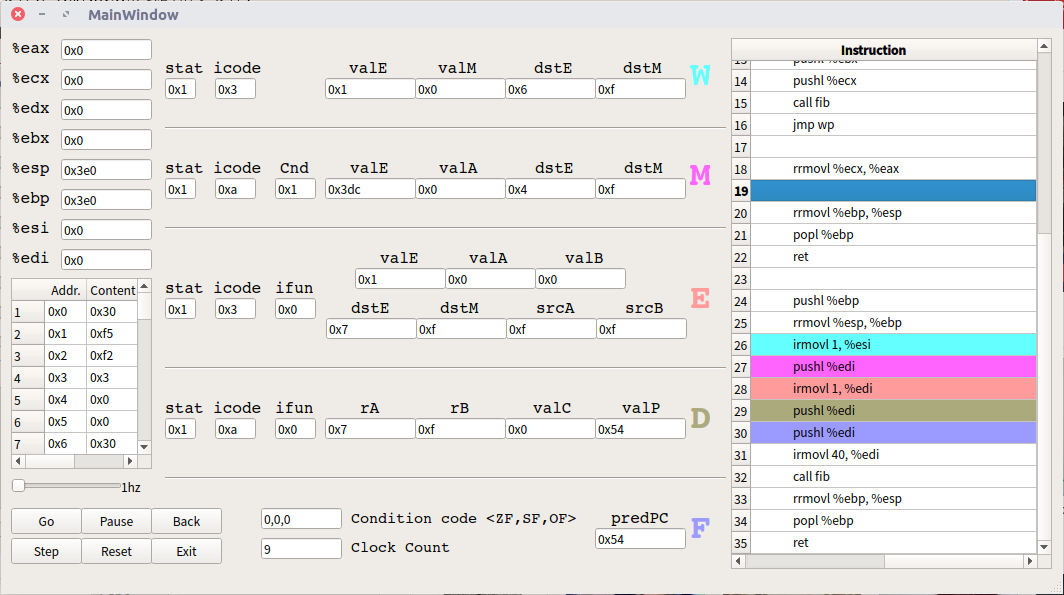
\includegraphics[width=0.9\textwidth]{pasted3}
\par\end{centering}
\caption{Y86Simulator 程序界面}

\end{figure}


\subsection{界面实现}

界面实现上采用了Qt,Qt是一个C++的库,因此界面程序可以直接调用内核部分产生的代码。对于界面程序来说,内核部分的所有变量都是可见的。因此每个时刻将要显示什么就直接读取代码里面相应的变量就可以了。

并且使用QtCreator编写界面十分直观。界面设计可以直接拖空间就可以。每个空间在代码上体现的就是一个个对象。

\subsubsection{每个流水线寄存器的显示}

与内核的沟通用一句\#include <pipe.h>就可以实现了。

在每一个Clock Cycle,读取pipe.h内部相应的变量,刷新相应的QLineinput上面显示的值就可以了。

\subsubsection{每个指令代码的显示}

使用QTableWidget显示每一句指令。在读入.yo文件时,预处理出每个指令开头地址与所在行数的对应关系。并显示在QTableWidget中。

为了跟踪每一条语句目前的执行阶段,在每一个阶段的寄存器中附带地传递了一个值begin,表示当前时刻此阶段通过的指令所在的地址,这样我们就知道每一条语句目前处于流水线的何种阶段。在每一个Clock
Cycle,刷新对应QTableWidget行的颜色为对应阶段所代表的颜色。

\subsubsection{每个内存值的显示}

同样使用QTableWidget显示每一个内存值。这里我们查看的是每一个字节的值。显示的时候只需要到内核部分代码中的HardwareUnits中的Memory结构体中查看数组的值就可以了。

\subsubsection{前进、暂停、后退等实现}

我们只需要在Qt中将前进、暂停等按钮的按下事件与内核部分处理一步的函数绑定在一起就可以。

关于后退的实现:我们在代码中存储了每一个ClockCycle下CPU内所有的状态。因此,每一次后退,我们只需要将CPU状态恢复到上一个Clockcycle即可。

\section{内核说明}

\subsection{支持指令:}
\begin{enumerate}
\item nop halt ret
\item rrmovl irmvol rmovl mrmovl
\item pushl popl
\item opl cmpl iropl
\item jxx call
\end{enumerate}
对任意的y86指令有效。

\subsection{冒险问题的解决:}

数据冒险:

转发:通过流水线寄存器+一些额外的数据通路和逻辑选择单元,将前面指令所未完成的写通过wire转发,从而知道最新的值,能使当前指令通过流水线寄存器而不需要任何的暂停。能解决绝大部分的冒险问题。

控制以及数据冒险:

完备的流水线控制逻辑。

主要需要解决的问题:
\begin{itemize}
\item 处理return:此时流水线必须暂停知道写回阶段。
\item 加载/使用冒险:在一条从存储器(内存)中读出一个值的指令和一条使用该值的指令之间,流水线必
\item 须暂停一个周期。
\item 错误预测的条件分支:需要撤销掉错误的指令
\item 异常:当指令导致异常,需要禁止后面的指令更新程序员可见的状态\&停止执行
\end{itemize}
具体的处理方法:
\begin{center}
\begin{tabular}{|c|c|c|c|c|c|}
\hline 
条件 & Fetch & Decode & Execyute & Memory & WriteBack\tabularnewline
\hline 
\hline 
处理RET & 暂停 & 气泡 & 正常 & 正常 & 正常\tabularnewline
\hline 
加载/使用冒险 & 暂停 & 暂停 & 气泡 & 正常 & 正常\tabularnewline
\hline 
预测错误的分支 & 正常 & 气泡 & 气泡 & 正常 & 正常\tabularnewline
\hline 
\end{tabular}
\par\end{center}

相关冒险的测试代码:

\begin{lstlisting}
  // Ret Hazard  
    0x000: 30f340000000 | 	irmovl mem,%ebx
    0x006: 504300000000 | 	mrmovl  0(%ebx),%esp 
    0x00c: 90           | 	ret		   
    0x00d: 00           | 	halt
    0x00e: 30f605000000 | rtnpt:  irmovl $5,%esi  
    0x014: 00           | 	halt
    0x040:              | .pos 0x40
    0x040: 50000000     | mem:	.long stack  0x050:             
    0x050:              | .pos 0x50
    0x050: 0e000000     | stack:	.long rtnpt  

  //Mispredicted Branch:
    0x000: 6300         | xorl %eax, %eax
    0x002: 7413000000   | jne target
    0x007: 30f202000000 | irmovl $2, %edx
    0x00d: 30f303000000 | irmovl $3, %ebx
    0x013:              | target:
    0x013: 30f001000000 | irmovl $1, %eax
    0x019: 00           | halt
    
  //Data Hazard:
    0x000: 30f0e8030000 | irmovl $1000, %eax
    0x006: 30f39a020000 | irmovl $666, %ebx
    0x00c: 403000000000 | rmmovl %ebx, (%eax)
    0x012: 501000000000 | mrmovl (%eax), %ecx
    0x018: 2012         | rrmovl %ecx, %edx
    0x01a: 00           | halt
\end{lstlisting}


\subsection{­ 新增指令(Bonus)}

cmpl,iropl和ircmpl。

cmpl: 寄存器值与寄存器值的比较

iropl: 立即数与寄存器之间的运算并赋值到寄存器中(包括 add sub and xor)

ircmpl: 立即数与寄存器之间的比较

具体的处理方法:

\begin{lstlisting}
  //cmpl rA, rB
  Fetch: icode:ifun<-M1[PC]   rA:rB<-M1[PC+1]  valP <-PC + 2
  Decode: valA<-R[rA]  valB<-R[rB]
  Execute: valE<-valB - valA   Set CC
  Memory:
  Writeback:
  PC update: PC<-valP

  //iropl V, rB
  Fetch: icode:ifun<-M1[PC]   rA:rB<-M1[PC+1]  valC<-M4[PC+2]   valP<-PC + 6
  Decode: valB<-R[rB]
  Execute: valE<-valB OP valC   Set CC
  Memory:
  Writeback: R[rB]<-valE
  PC update: PC<-valP

  //ircmpl V, rB
  Fetch: icode:ifun<-M1[PC]   rA:rB<-M1[PC+1]  valC<-M4[PC+2]   valP<-PC + 6
  Decode: valB<-R[rB]
  Execute: valE<-valB - valC   Set CC
  Memory:
  Writeback:
  PC update: PC<-valP
\end{lstlisting}


\subsection{效率上的优化(Bonus)}

课程中中PIPE对ret指令的处理:将ret的“下一条”指令阻塞在取指阶段,直至上一条指令访存阶段结束(即进入写回阶段),这样做有一个缺陷就是:效率不高,因为对于每次的ret,都会出现三个周期的时间的浪费。

因此我们采取了这样的做法:加入程序员不可见的硬件栈,对ret的返回地址在Fetch阶段进行预测,这样就没有暂停。

在call的时候将下一条指令压入栈中;在ret的时候将栈顶弹出并作为ret的返回地址的预测值。这样做的原理是一般情况下函数的调用和返回是成对出现的,基本上都能预测正确。但是这样子做是可能会出现预测错误的情况的,比如这两种情况:
\begin{enumerate}
\item jxx(条件跳转)预测错误带来的连锁效应。
\item 有时候会出现手动压返回地址的情况,没用call就ret。
\end{enumerate}
所以我们需要一个恢复机制:

对ret预测正确性的判定,可以在ret完成访存阶段(Memory)后得到。如果预测错误,那么给M,E,D流水线寄存器插入bubble信号来撤销错误的操作即可。

还有一个问题,就是如果ret返回值预测错误的话,我们加入的硬件栈会被污染。所以我们需要一个可以快速恢复的栈:每次操作只新建,不修改(其实是一个树的结构)

\begin{figure}[h]
\begin{centering}
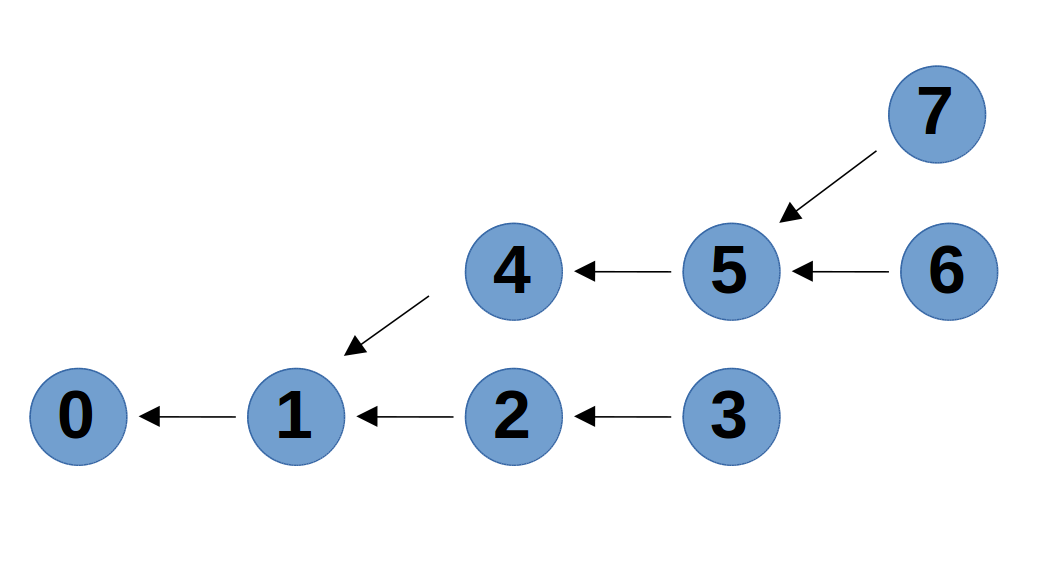
\includegraphics[width=0.8\textwidth]{pasted1}
\par\end{centering}
\caption{恢复机制示意图\label{fig:=006062=00590D=00673A=005236=00793A=00610F=0056FE}}

\end{figure}

如图\ref{fig:=006062=00590D=00673A=005236=00793A=00610F=0056FE}所示:在时刻1,2,3,5,6对栈进行的是push操作,在时刻4进行的是pop操作,在时刻7没有操作。如果需要恢复,只需要将时间戳­-3(ret预测错误)或者-­2(jxx预测错误)即可。 

还有一个缺陷:由于最早的错误指令会执行完Execute阶段,程序员可见的条件码可能会被污染,但是注意到 SelectPC在需要用到条件码的时候,条件码已经被正确的指令更新了,不会影响整体的逻辑(不过这的确是个
缺陷,其实如果把条件码也改成可持久化的就可以解决这个问题)

测试结果(递归求fibonacci数列第n项):
\begin{center}
\begin{tabular}{|c|c|c|c|c|}
\hline 
初始值 & 10 & 20 & 30 & 40\tabularnewline
\hline 
\hline 
加入硬件栈前 & 217(周期) & 417 & 617 & 817\tabularnewline
\hline 
加入硬件栈后 & 184 & 354 & 524 & 694\tabularnewline
\hline 
\end{tabular}
\par\end{center}

可以看出效率提升了很多。

\section{lab过程和感想}

王鹏:在这次的project中,我负责的是kernel部分。

最开始对于这个kernel我毫无头绪,不知道从何下手,所以只能按照自己的理解先把大概的框架弄出来,后来根据教材提供的hcl语言和pipeline的配图,了解了每个单元具体所做的事情以后就比较好些了。因为我对于每个阶段的pipeline都开了一个struct,中间过程中有有些地方是调用当前的pipe(组合逻辑)还是上一个阶段的pipe(时序逻辑)我没有分得太清楚,结果调bug调了很长的时间,我认为这是不应该的,最好是一开始就把组合逻辑和时序逻辑分清楚,这样就不会出那么多bug。后期的难点是控制逻辑的设计,因为这是一个很烧脑的事情,要自己先模拟好冒险的情况和处理方法,才能清楚自己在写什么东西。

​但是光完成教程上的东西是远远不够的,于是我想在写好的pipe的基础上加入一些其他的东西。首先是加入新的指令,cmpl这iropl这两个指令加上去不算很难,后面我还想加入一个比较奇葩的swapl(交换两个寄存器的值)的操作,但是后面发现register
files只有一个写端口,后来这个想法就报废了。

​然而我在书上翻到了一个扩展阅读,里面介绍了现代的cpu对于call/ret操作是有一个专门的硬件栈进行预测的,我想了想觉得这是个很好的feature,而且感觉是可以实现的。于是我尝试去实现了这个功能,后来还调了整整一天的bug才把教材提供的测试文件们给调过去。最终测试是效率的确提高了不少,非常开心。

总而言之,我觉得这次的y86-simulator的设计非常的有意思,而且能让我们更加深入地理解计算机系统,虽然中间过程很坎坷,但是这对于我而言是非常有意义的事情。

卢力韬:在这次的project中,我负责的是界面部分。并且还实现了一个Y86的as(编译器)(虽然后来没用到……)。

这次写PJ也是我第一次写有界面的程序。刚开始我也不知道如何实现一个界面。通过网上查找一些资料,最后选定了Qt库。在编写的过程中,要看到很多队友的代码,以及有稍稍修改队友的代码。这对我也是一种比较新的体验,因为要将自己的代码嵌入到别人代码中。还不能将别人和自己的代码改错。特别提一下,因为是两个人写代码,我们用github实现我们代码的同步(虽然用的还不是很熟练)。

自己实现的Y86编译器也带给我挺多收获,首先,因为程序输入格式约束并不严格,所以程序要应对所有的情况,所以编写起来比较繁,后来看到有人用regex先预处理一下输入,这是一个很好的方法。

通过这次写PJ,我学习了一下Qt的用法。并且因为要看懂队友的代码,我们也复习了很多CPU流水线的知识。总的来说,这次PJ还是很有意思的。
\end{document}
